\begin{figure}
    \begin{center}
    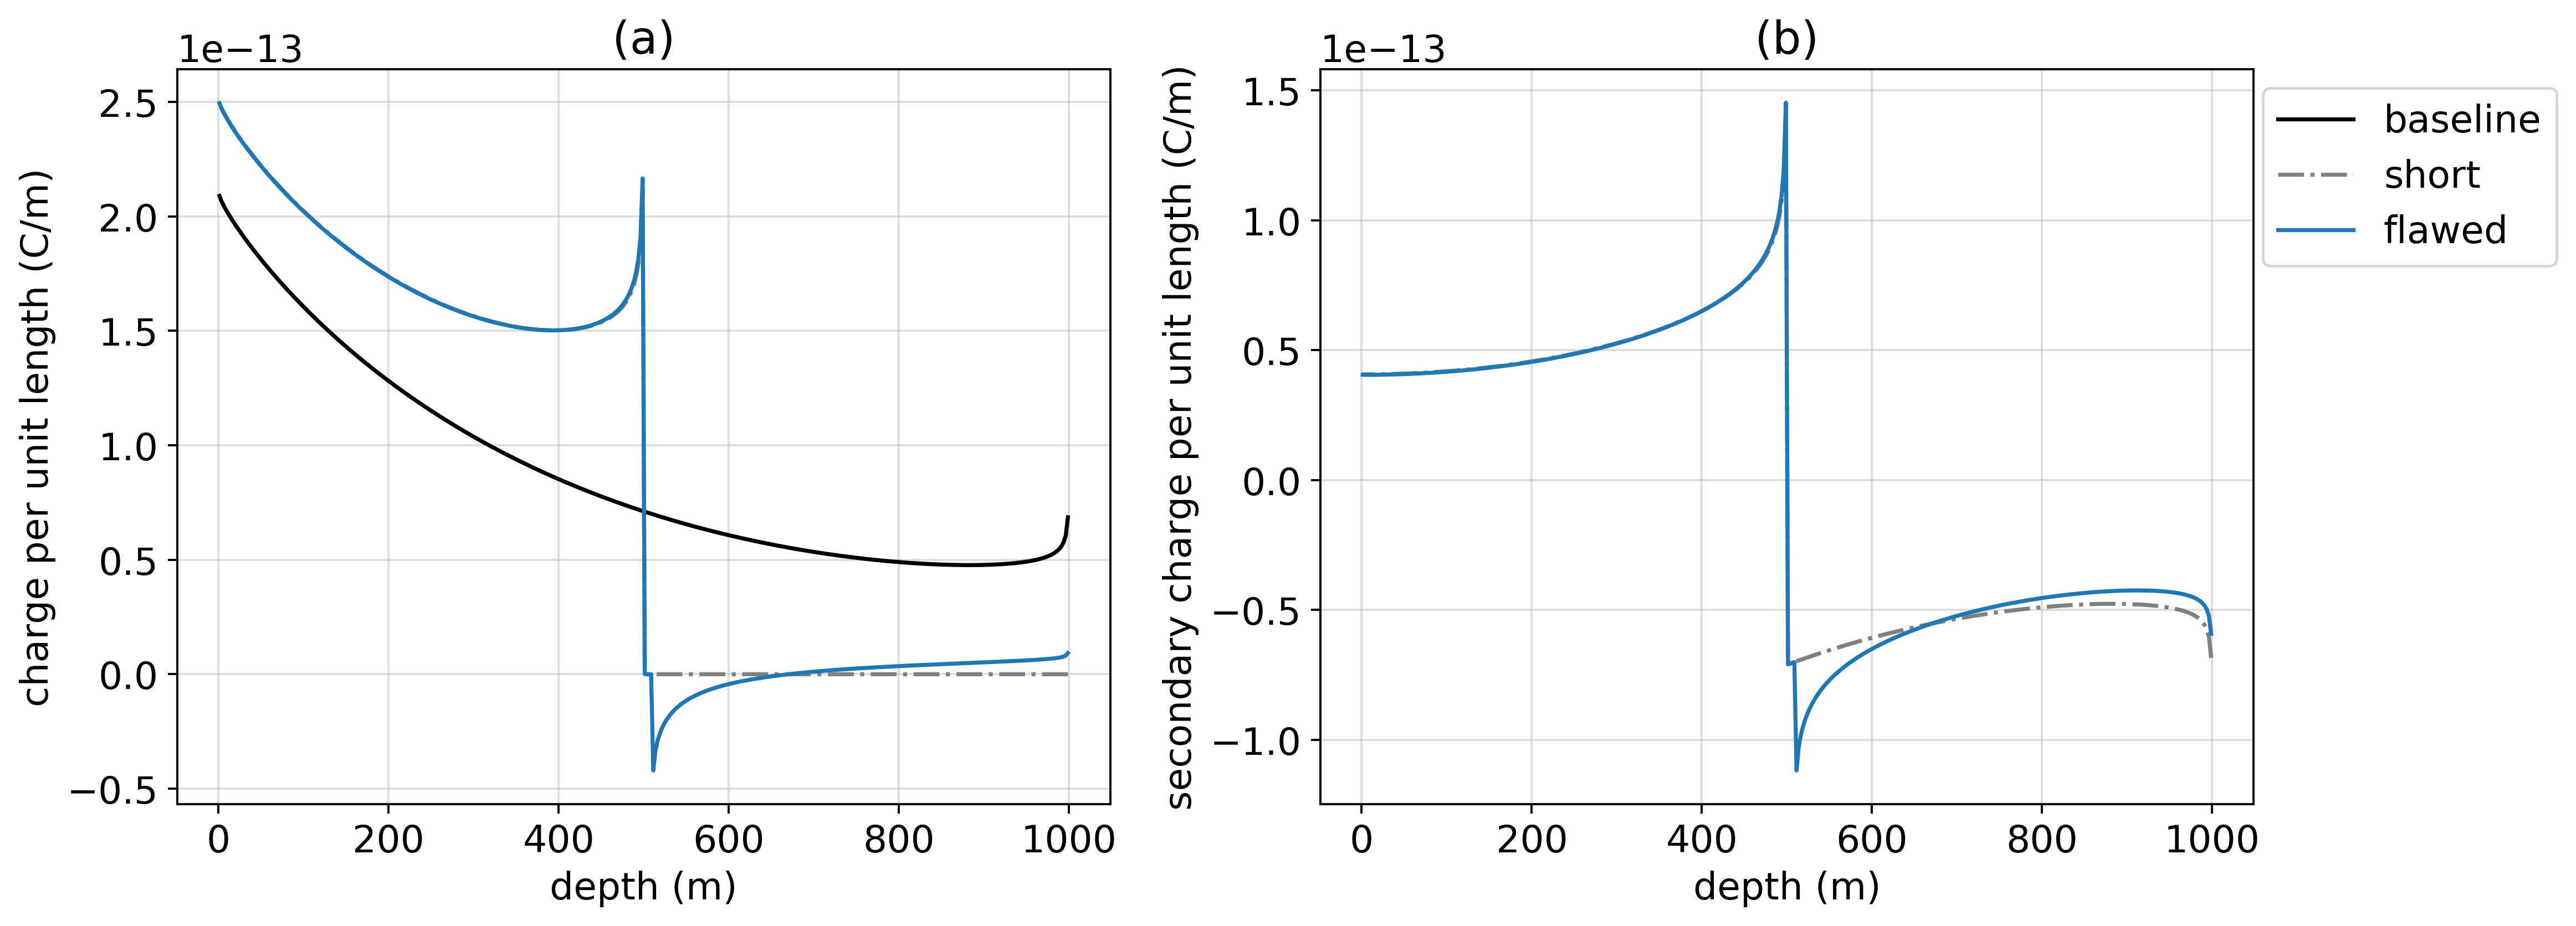
\includegraphics[width=\textwidth]{figures/casing_charge.png}
    \end{center}
\caption{
    (a) Charge along the length of the intact well (black),
    a 500m well ( ``short'', grey dash-dot), and
    a well with a 10m flaw at 500m depth (blue),
    in a top-casing DC resistivity experiment.
    (b) Secondary charge along the flawed and short wells. The primary is
    defined as the electric field due to the 1000m long intact well. The return electrode
    is 2000m away from the well.
}
\label{fig:casing_charge}
\end{figure}
